\subsection{Queue}
The queue will handle keeping track of requests made and their responses in the order that they are made.

\begin{figure}[h!]
	\centering
 	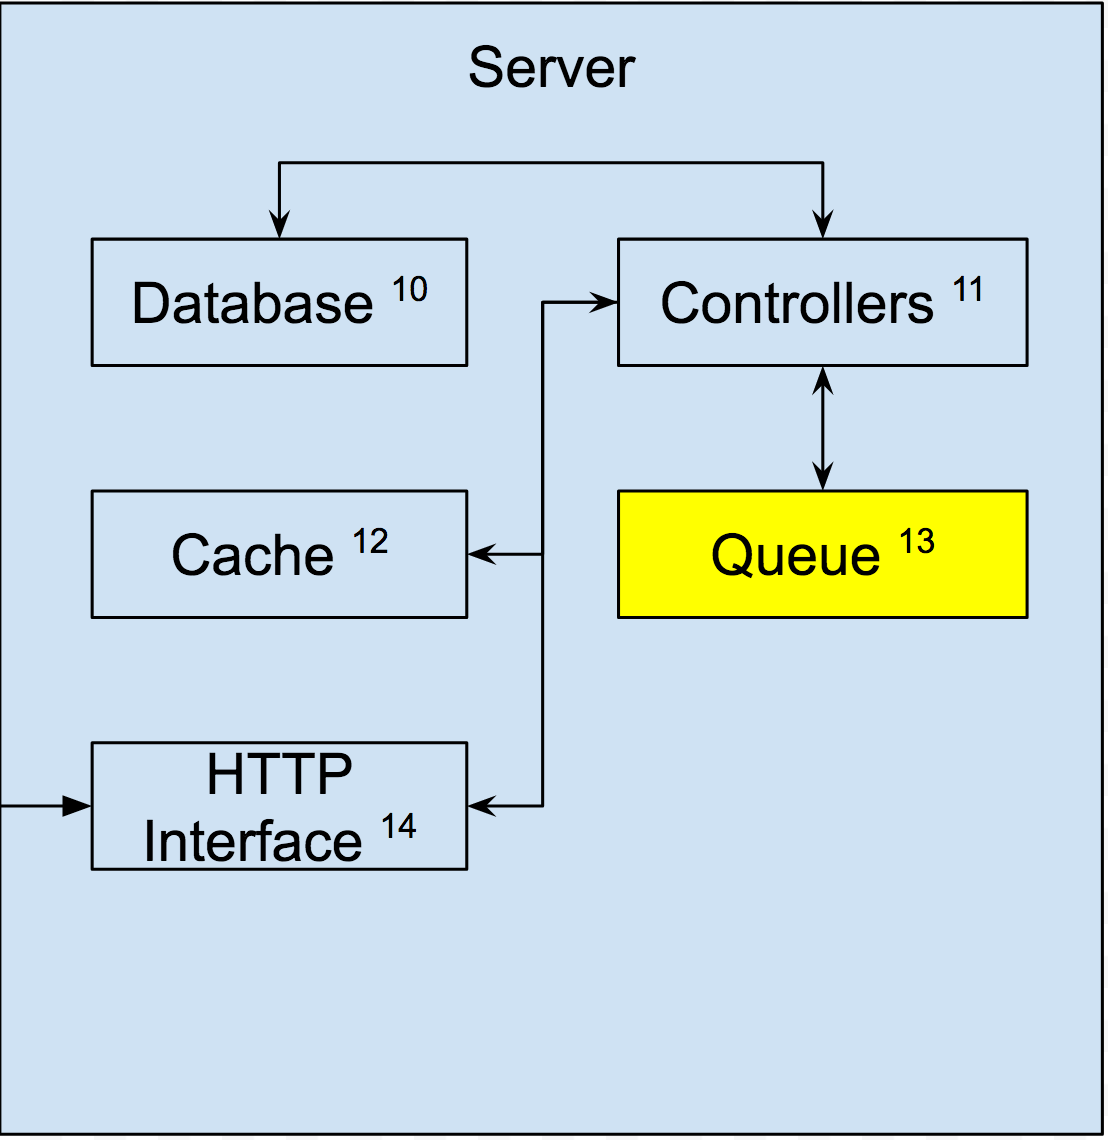
\includegraphics[width=0.60\textwidth]{images/server/server_queue.png}
 	\caption{Queue subsystem}
\end{figure}

\newpage

\subsubsection{Subsystem Hardware}
This project is primarily software, but we will be hosting our live site using Heroku, so whatever hardware they are using for their servers is our hardware.

\\
\subsubsection{Subsystem Operating System}
This project is primarily software, but we will be hosting our live site using Heroku, so whatever OS they are using for their servers (usually UNIX systems such as macOS, Linux) is our OS.

\\
\subsubsection{Subsystem Software Dependencies}
The queue will be implemented as a normal queue (First In First Out) in our chosen programming language, and as such, will not have any dependencies.

\\
\subsubsection{Subsystem Programming Languages}
The programming language to be used will be Go. Go is a modern and great programming language to work with and will satisfy our needs to provide an implementation of a request queue.

\\
\subsubsection{Subsystem Data Structures}
We will be utilizing a regular queue for our request queuing. The data structure used for the queuing will be arrays, and each request that comes through will be appended to our arrays. Then we will be popping the arrays from the front when we are ready to handle the next request.

\\
\subsubsection{Subsystem Data Processing}
The data will be processed in the same way a queue processes data: "First In First Out".

\newpage